\documentclass{article}
\usepackage[a4paper, total={6.3in, 9.6in}]{geometry}
\usepackage[utf8]{inputenc}
\usepackage[french]{babel}
\usepackage{graphicx}
\usepackage{graphics}
\usepackage{colortbl}
\usepackage[T1]{fontenc}
\usepackage{amsmath}
\usepackage{hyperref}
\usepackage{array}
\usepackage{amssymb}
\usepackage{colortbl}
\usepackage{color}
\usepackage{listings}
\usepackage{xcolor}
\usepackage{array}
\usepackage{float}
\usepackage{amsfonts}
\usepackage{fancyhdr}
\usepackage{wrapfig}

\setcounter{topnumber}{2}
\setcounter{bottomnumber}{2}
\setcounter{totalnumber}{4}
\renewcommand{\topfraction}{0.85}
\renewcommand{\bottomfraction}{0.85}
\renewcommand{\textfraction}{0.15}
\renewcommand{\floatpagefraction}{0.8}
\renewcommand{\textfraction}{0.1}
\setlength{\floatsep}{5pt plus 2pt minus 2pt}
\setlength{\textfloatsep}{5pt plus 2pt minus 2pt}
\setlength{\intextsep}{5pt plus 2pt minus 2pt}

\hypersetup{
    colorlinks=true,
    linkcolor=black,
    filecolor=magenta,
    urlcolor=cyan,
    pdftitle={Overleaf Example},
    pdfpagemode=FullScreen,
    }

\title{LEPL1252 - Projet 0}
\author{Matya Aydin \& Thomas Debelle}
\date{Novembre 2023}

\begin{document}

\maketitle

\section{Fonctionnement}


Ajouter les 3 états d'exécution avec un diagramme et mettre les informations de l'algo

\subsubsection{Structure de la mémoire}

\begin{wrapfigure}{r}{0.5\textwidth}
    \centering
    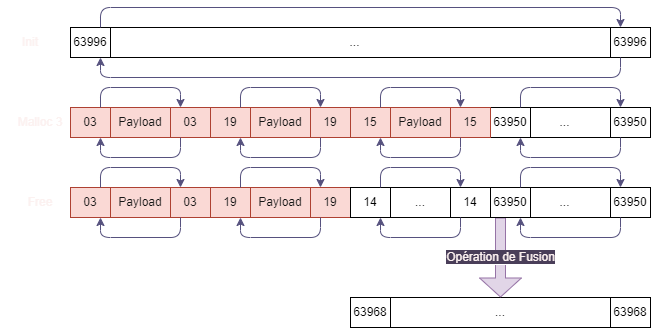
\includegraphics[width=0.5\textwidth, trim = {0 1.6cm 0 1.5cm}, clip]{fonctionnement.png}
    \caption{Structure de la mémoire}
    \label{fct}

\end{wrapfigure}

Autour de chaque morceau de mémoire se trouve des informations sur la taille de ce dernier. À la création, on indique donc qu'il y a 63998 octets disponibles. Ce nombre est écrit au début et à la fin de chaque morceau (les avantages de cette structure sont abordés aux sections \ref{free} et \ref{perf}). Ci-contre, une représentation abstraite de la mémoire.

\subsubsection{Malloc}
Notre implémentation de `malloc` est la suivante, on met de part et d'autre des cases des données la taille disponible. On alloue que des tailles paires ainsi on peut utiliser le bit de poids faible pour indiquer si les blocs sont libres ou occupés. Donc si c'est un nombre pair par exemple 4, il y a donc 4 emplacements libres de 8 bits. Si ce chiffre était 5, cela signifierait qu'il y a 4 octets mais qu'ils ont été alloués par malloc.\\
On commence par chercher le premier ensemble de blocs qui puissent accueillir la taille désirée par l'utilisateur. On commence au début de notre Heap à chaque fois. On va donc partitionner un ensemble de blocs en 2 plus petits ensembles. Le premier des deux a la taille désirée par l'utilisateur et le deuxième est le reste des blocs.\\
Il est important de noter qu'à chaque fragmentation de notre mémoire, 4 octets de méta-données sont requis.

\subsubsection{Free}
\label{free}
Notre free va éviter la fragmentation de la mémoire. En effet, on regarder si les fragments de mémoire à droite et à gauche de celui qu'on veut libérer sont libres. Si c'est le cas on va donc regrouper nos fragments en un seul comme montré à la figure \ref{fct}.\\
Nous ne remettons pas les octets fraîchement libérés à 0 pour éviter une consommation de ressources inutiles. On ne fait rien si l'utilisateur essaye de libérer des octets déjà libres.


\section{Discussion \& Performances}
\label{perf}

\subsubsection*{Motivation du choix d'algorithme}
Notre politique first fit ...


\end{document}